\section{Results}
\label{sec:results}

%Performance Evaluation, Results, Discussion}

\textit{owners: Evan: graphs, All: interpretation (2.75 pages)}

\subsection{Scaling on Single Node}
  \label{sxn:results1}


   
  \vspace*{0.1in}

      In Table~\ref{tab:single_node}, we show the benefits of various
      optimizations described in
      Sec.~\ref{sxn:single_node_opt} on a single-node of our Spark system. 
      The test matrix $\mathcal{A}$ has {\it{m}} = 1.95M, {\it{n}} = 128K,
      {\it{s}} = 0.004, and {\it{nnz}} = 10$^9$. The rank parameter,
      {\it{k}} = 32. We started with a parallelized implementation,
      without any of the described optimizations, and measured the
      performance (in terms of time taken). We first implemented the
      multi-core synchronization scheme, wherein a single copy of the
      output matrix is maintained across all the threads (for the matrix multiplication).
      This resulted in a speedup of around 6.5X, primarily due to
      the reduction in the amount of data traffic between the
      last-level cache and main memory (there was around 19X measured reduction
      in traffic). We then implemented our cache blocking scheme,
      primarily targeted towards ensuring that the output of the
      matrix multiplication resides in the caches (since it is
      accessed and updated frequently). This led to a further 2.4X
     reduction in run-time, for an overall speedup of around 15.6X.

     Once the memory traffic was optimized for, we implemented our
     SIMD code, by vectorizing the element-row multiplication-add
     operations (described in detail in Sec.~\ref{sxn:single_node_opt}). 
     The resultant code sped up by a further 2.6X, for an overall
     speedup of 39.7X. Although the effective SIMD width
 ($\mathcal{S}$ = 4), there are overheads of address computation,
 stores, and not all computations were vectorized (QR code is still
 scalar).


 
  \begin{table}
  \begin{center}
  \begin{tabular}{ |c|c| } 
  \hline
  Single Node Optimization & Overall Speedup\\
  \hline
  Original Implementation & 1.0  \\
  Multi-Core Synchronization & 6.5 \\
  Cache Blocking & 15.6 \\
  SIMD & 39.7 \\
  \hline

  \end{tabular}
  \end{center}
  \caption{Single node optimizations to the CX C implementation and
  the subsequent speedup  each additional optimization provides.}
  \label{tab:single_node}
  \end{table}
 



  \subsection{Scaling across Multiple Nodes}
  \textcolor{red}{Mike R, Jatin: we need a narrative here}

  \subsubsection{CX Spark Phases}
  Our implementations of CX and PCA share the \textsc{RandomizedSVD} subroutine, which accounts for the bulk of the runtime and all of the distributed computations.
  The execution of \textsc{RandomizedSVD} proceeds in four distributed phases listed below, along with a small amount of additional local computation.
  \begin{enumerate}
      \item \textbf{Load Matrix Metadata}
         The dimensions of the matrix are read from the distributed filesystem to the driver.
      \item \textbf{Load Matrix}
         A distributed read is performed to load the matrix entries into an in-memory cached
         RDD containing one entry per row of the matrix.
      \item \textbf{Power Iterations}
         The \textsc{MultiplyGramian} loop on lines 2-5 of
         \textsc{RandomizedSVD} is run to compute an approximation $Q$
         of the dominant right singular subspace.
       \item \textbf{Finalization (Post-Processing)}
         Right multiplication by $Q$ on line 7 of \textsc{RandomizedSVD} to compute $C$.
  \end{enumerate}

  \subsubsection{Empirical Results}

    \begin{figure} [H]
    \begin{centering}
    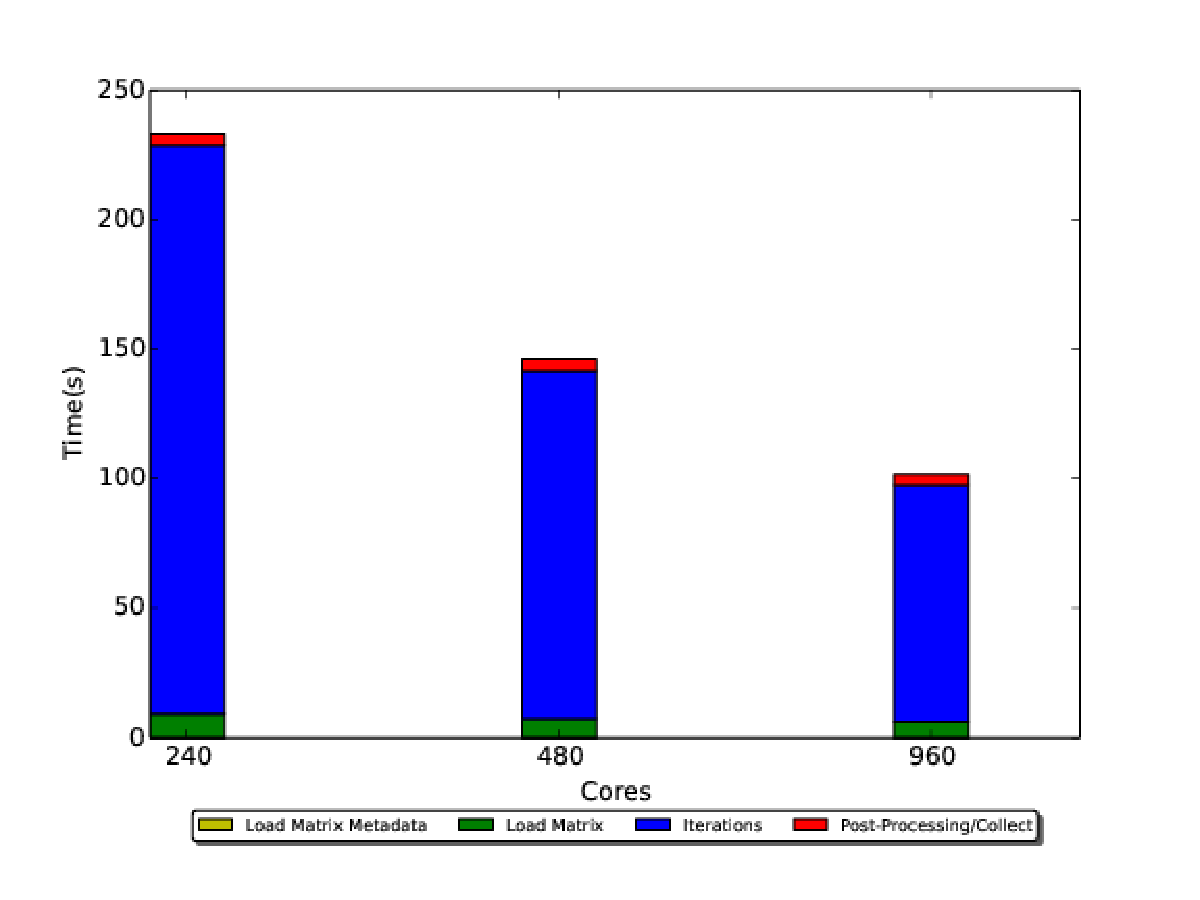
\includegraphics[scale=0.4]{images/CX_Strong_Scaling_Rank_32_Partitions_default.pdf}
    \end{centering}
    \caption{ Strong scaling for the 4 phases of CX on an XC40 for 100GB dataset at rank 32 and default partitioning as concurrency is increased.} 
    \label{fig:xc40scaling}
    \end{figure} 

Figure~\ref{fig:xc40scaling} shows how the distributed Spark portion of our code scales as we add additional processors.  We considered 240, 480, and 960 cores.  An additional doubling (to 1920 cores) would be ineffective as there are only 1654 partitions, so many cores would remain unused.  In addition, with fewer partitions per core there are less opportunities for load balancing and speculative reexecution of slow tasks.

When we go from 240 to 480 cores, we achieve a speedup of approximately 1.6x from doubling the cores: 233 seconds versus 146 seconds.  However, as the number of partitions per core drops below two, and the amount of computation-per-core relative to communication overhead drops, the scaling slows down (as expected).  This results in a lower speedup of approximately 1.4x (146 seconds versus 102 seconds) when we again double the core count to 960.

  \subsection{Comparison across Multiple Platforms}
  \label{sect:h2h}
    
    \begin{figure} [H]
    \begin{centering}
    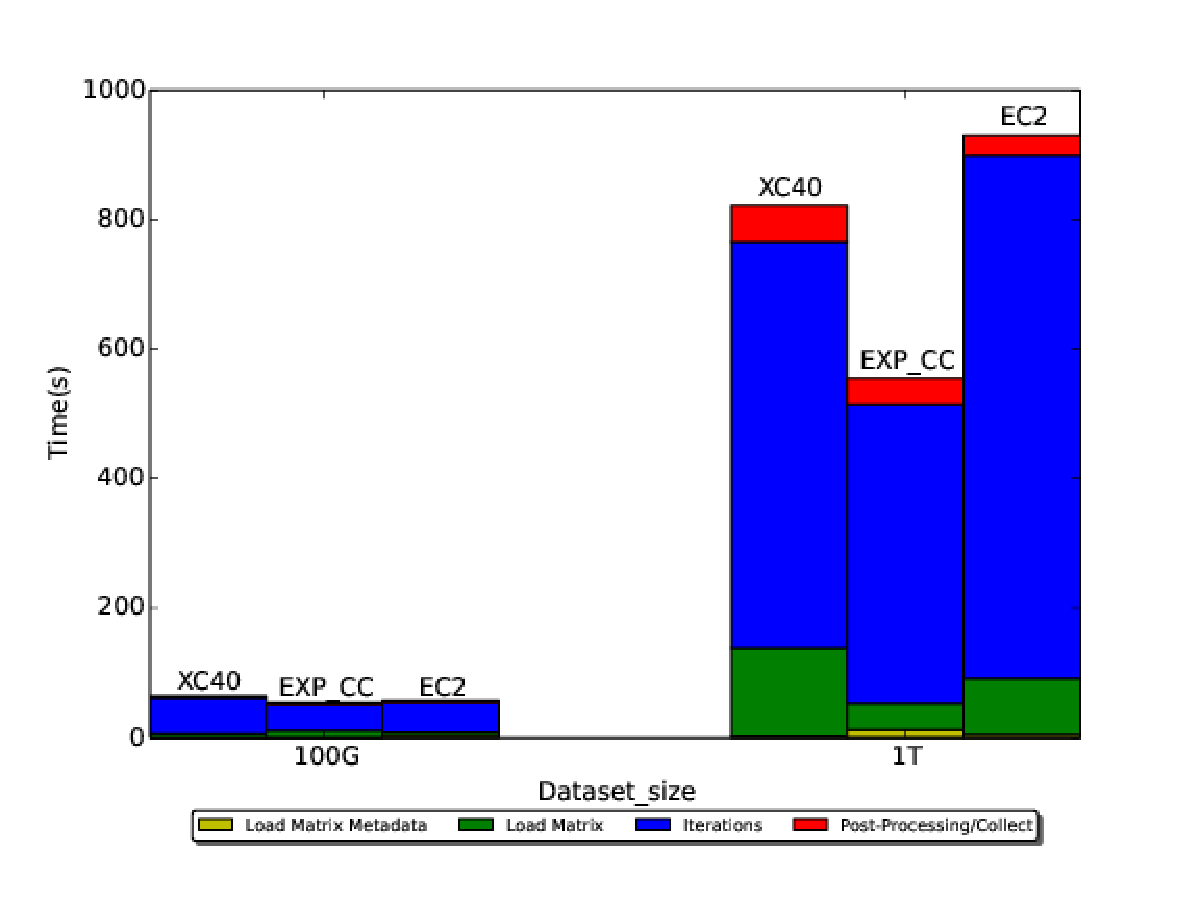
\includegraphics[scale=0.4]{images/CX_Size_Scaling_Rank_16_Partitions_default.pdf}
    \end{centering}
    \caption{ Run times for the various stages of computation for CX for two different dataset sizes for the three platforms using rank 16 and default partitioning for the given platform} 
    \label{fig:h2hrank16} 
    \end{figure}

    
      \begin{figure} [H]
    \begin{centering}
    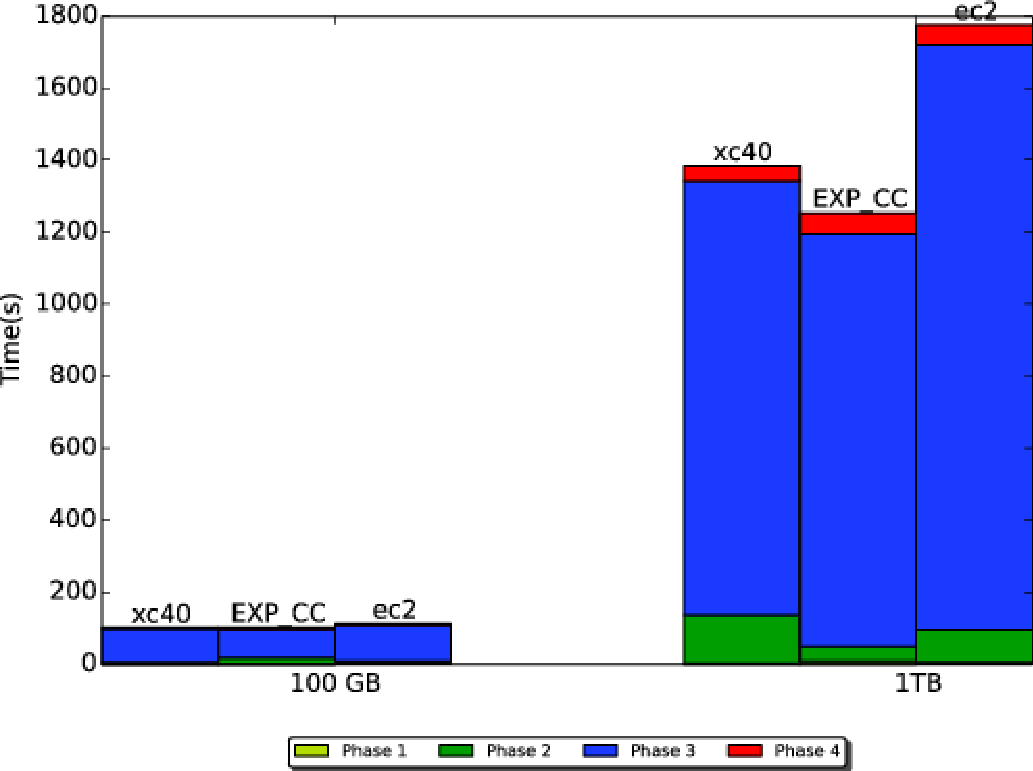
\includegraphics[scale=0.4]{images/CX_Size_Scaling_Rank_32_Partitions_default.pdf}
    \end{centering}
    \caption{ Run times for the various stages of computation for CX for two different dataset sizes for the three platforms using rank 32 and default partitioning for the given platform}
    \label{fig:h2hrank32} 
    \end{figure}
    
    \begin{table*}
    \begin{center}
    \begin{tabular}{| l | c | c | c | c | c | c | c |}
    \toprule
    \textbf{Platform} & \textbf{Rank} & \textbf{Total} & \textbf{Load} & \textbf{Time Per} & \textbf{Average} & \textbf{Average} & \textbf{Average} \\
                               & & \textbf{Runtime} & \textbf{Time} & \textbf{Iteration} & \textbf{Local} & \textbf{Aggregation} & \textbf{Network} \\
                               & & & & & \textbf{Task} & \textbf{Task} & \textbf{Wait} \\
    \midrule
    Amazon EC2 r3.8xlarge & 16 & 24.0 min & 1.53 min & 2.69 min & 4.4 sec & 27.1 sec & 21.7 sec \\
    \midrule
    Cray XC40 & 16 & 23.1 min& 2.32 min & 2.09 min &  3.5 sec & 6.8 sec & 1.1 sec \\
    \midrule
    Experimental Cray cluster & 16 & 15.2 min & 0.88 min & 1.54 min &  2.8 sec & 9.9 sec & 2.7 sec \\
    \midrule
    Amazon EC2 r3.8xlarge & 32 & 52.6 min& 1.57 min & 5.42 min &  8.7 sec & 60.1 sec & 48.7 sec \\
    \midrule
    Cray XC40 & 32 & 41.2 min & 2.28 min & 4.01 min &  7.5 sec & 25.0 sec & 15.4 sec \\
    \midrule
   Experimental Cray cluster & 32 & 35.8 min & 0.81 min & 3.82 min &  6.8 sec & 27.9 sec & 15.5 sec \\
   \bottomrule
    \end{tabular}
    \end{center}
    \caption{Total runtime for the 1 TB dataset, broken down into load time and per-iteration time. The per-iteration time is further broken down into the average time for each task of the local stage and each task of the aggregation stage.  We also show the average amount of time spent waiting for a network fetch, to illustrate the impact of the interconnect.}
    \label{tab:h2hres1TB}
    \end{table*}
    
Table~\ref{tab:h2hres1TB} shows the total runtime of CX for the 1 TB dataset on our three platforms.  The distributed Spark portion of the computation is also depicted visually in Figures~\ref{fig:h2hrank16} (rank 16) and~\ref{fig:h2hrank32} (rank 32).  All three platforms were able to successfully process the 1 TB dataset at rank 16 in under 25 minutes.  As the table and figures illustrate, most of the variation between the platforms occurred during the \texttt{MultiplyGramian} iterations.  Table~\ref{tab:hwspecs} shows the specifications of the three platforms. In this section, we explore how these difference relate to the performance of the matrix iterations.

  \begin{table*}
    \begin{center}
    \begin{tabular}{| l | c | c | c | c | c | c | c |}
    \toprule
    \textbf{Platform} & \textbf{Total Cores} & \textbf{Core Frequency} & \textbf{Interconnect} & \textbf{DRAM} & \textbf{SSDs} \\
    \midrule
    Amazon EC2 r3.8xlarge & 960 (32 per-node) & 2.5 GHz & 10 Gigabit Ethernet & 244 GiB & 2 x 320 GB \\
    \midrule
    Cray XC40 & 960 (32 per-node) & 2.3 GHz & Cray Aries\texttrademark & 252 GiB & None \\
    \midrule
    Experimental Cray cluster & 960 (24 per-node) & 2.5 GHz & Cray Aries\texttrademark & 126 GiB & 1 x 800 GB \\
    \bottomrule
    \end{tabular}
    \end{center}
    \caption{Specifications of the three hardware platforms used in these performance experiments.}
    \label{tab:hwspecs}
  \end{table*}

Spark divides each iteration into two stages.  The first \emph{local} stage computes each row's contribution, sums the local results (the rows computed by the same worker node), and records these locally-aggregated results.  The second \emph{aggregation} stage combines all of the workers' locally-aggregated results using a tree-structured reduction.  Most of the variation between platforms occurs during the aggregation phase, where data from remote worker nodes is fetched and combined.  In Spark, all inter-node data exchange occurs via \emph{shuffle operations}.  In a shuffle, workers with data to send write the data to their local scratch space.  Once all data has been written, workers with data to retrieve from remote nodes request that data from the sender's block manager, which in turns retrieves if from the senders local scratch space, and sends it over the interconnect to the receiving node.

Examining our three platforms, we notice two key hardware differences that impact shuffle operations.  First, both the EC2 nodes and the experimental Cray cluster nodes have fast SSD storage local to the compute nodes.  The Cray XC40, on the other hand, has no local block storage.  Thus it must emulate local storage with a remote Lustre filesystem.  The impacts of this can be somewhat mitigated, however, by leaving sufficient memory to store some of the scratch data in local RAM disk, and to locally cache some of the remote writes to Lustre.\footnote{This is an ideal usage of caching, since Spark assumes the scratch space is only locally accessible; thus we are guaranteed that the only node that reads a scratch file will be the same node that wrote it.}  Second, the Cray XC40 and the experimental Cray cluster both communicate over the HPC-optimized Cray Aries interconnect, while the EC2 nodes use 10 Gigabit Ethernet.  

We can see the impact of differing interconnect capabilities in the Average Network Wait column in Table~\ref{tab:h2hres1TB}.   These lower average network wait times explain why the two Cray platforms outperform the EC2 instance (with the experimental cluster achieving a speedup of roughly 1.5x over EC2).  The XC40 is still slightly slower than the experimental Cray platform, however, in particular at rank 16.  This can be understood by looking at the Maximum Aggregation Task and Maximum Network Wait columns.  \textbf{(NOTE: Verify that this is correct when Evan adds max data to Google Docs table, and add these to paper table.)}  Despite having lower average task and network wait times, the iteration time is actually higher because we have to synchronize after each iteration and wait for the slower tasks to complete.  These slow running tasks are indicative of data that was written to the remote Lustre filesystem and not locally cached (or subsequently evicted from the local cache).


  

  \subsection{Comparison of CX, PCA, RPCA quantitatively \textcolor{red}{Alex: please insert results here} }
    \begin{itemize}
      \item (for 100GB sized dataset on EC2)
      \item runtime vs. accuracy?
      \item show distinction b/w cx, pca
    \end{itemize}

  \subsection{Science plot for PCA, CX}
    \begin{figure} [H]
    \begin{centering}
    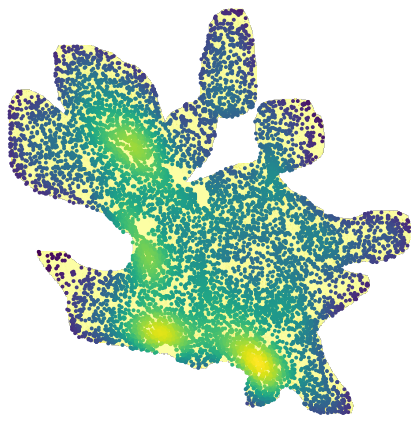
\includegraphics[width=\linewidth]{images/cx_spatial.png}
    \end{centering}
    \caption{Plot of 10000 locations sampled by leverage score.
      Color indicates the density of samples in each area as computed by a Gaussian kernel density estimate.}
    \label{fig:cx_spatial}
    \end{figure} 

    \begin{figure} [H]
    \begin{centering}
    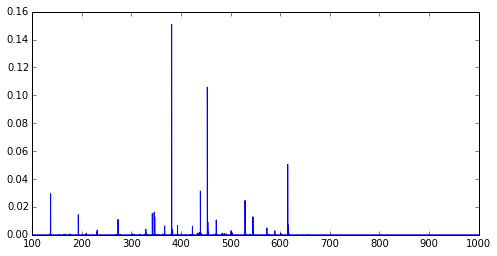
\includegraphics[width=\linewidth]{images/cx_ions.png}
    \end{centering}
    \caption{Normalized leverage scores (sampling probabilities) for m/z marginalized over $\tau$.
      Three narrow regions of m/z account for 59.3\% of the total probability mass.}
    \label{fig:cx_ions}
    \end{figure} 


  \subsection{Lessons Learned}
  \label{sect:lessons}
  
  The differences in performance between the Cray\textregistered~XC40\textsuperscript{\tiny\texttrademark} system~\cite{alverson2012cray,craycascadesc12} and the experimental Cray cluster point to optimizations to Spark that could improve its performance on HPC-style architectures.  The two platforms have very similar configurations, with the primary difference being the lack of local persistent storage on the XC40 nodes.  As described in Section~\ref{sect:h2h}, this forces some of Spark's local scratch space to be allocated on the remote Lustre file system, rather than in local storage.  To mitigate this, and keep more of the scratch data local, we propose the following future investigations:
\begin{itemize}
\item Spark is currently inefficient in cleaning up its local scratch space.  In particular, shuffle data is not immediately cleaned up after a shuffle completes.  This makes fault recovery more efficient, but results in higher storage requirements for scratch space.  If clean up was more efficient, it would be more feasible to fit all of the scratch data in a local RAM disk and not rely on Lustre at all.
\item Spark does not currently allow you to configure primary and backup scratch directories.  Instead you list all scratch directories in a single list, and it distributes data in a round round fashion between them as long as space is available.  You can bias it towards one storage device (e.g., RAM disk vs. Lustre) by listing multiple directories on the preferred device.  Ideally, though, we would like to use a RAM disk (or other local storage) exclusively unless and until it fills, and only switch to Lustre directories if necessary.
\item Spark does not allow you to specify that a scratch directory is globally accessible.  Thus non-cached data is stored to the remote Lustre directory by the sender, and then later retrieved by the sender and sent to the receiver.  This wastes a step, since the receiver could easily fetch the data directly from Lustre (or any other global file system).
\item Alternatively, a push model of communication (as opposed to the current pull model) might be possible - however this would have implications for reliability and handling of very large data sets.\footnote{Storing the shuffle data to a large persistent block storage device, and only sending it as needed, allows Spark to easily shuffle more data than could fit in the remote buffers.  In a push-based model, extra logic and synchronization would be necessary to ensure that the remote buffers do not overflow.}
\end{itemize}


